% contexte
Le présent document se concentre sur un problème d'affichage graphique;
étant donné un point de vue, il s'agit représenter ce qu'il voit en
prenant en compte le fait que certains objets en cachent d'autres.
Il s'agit d'afficher à partir d'un ensemble de segments dans le
plan une représentation en une dimension de ce que voit le point de vue
(voir les figures
\ref{intro:ill}, \ref{intro2:ill}).

L'algorithme du peintre est la solution employée pour résoudre le problème et
la structure de donnée associée, l'arbre BSP
(\emph{binary space partition tree}), est étudiée dans ce document.

Une implémentation en Java des arbres BSP et de l'algorithme
du peintre a été réalisée, grâce à laquelle plusieurs
heuristiques de construction d'arbres BSP ont pu être testées et
comparées à l'aide de tests sur machine.

Le mode d'emploi de l'application est également fourni dans ce rapport.

\begin{figure}[!h]
  \begin{center}
    \caption{Visualisation d'une scène par un \oe{}il}%
    \label{intro:ill}
    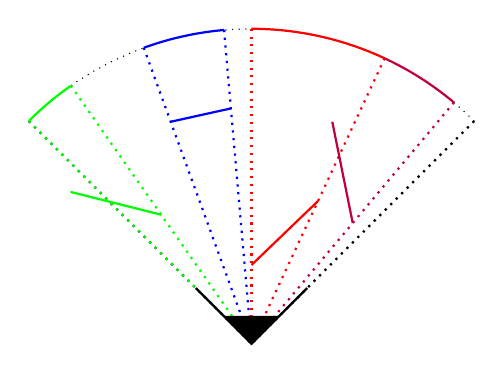
\begin{tikzpicture}[scale=1, thick]
      \begin{scope}[rotate=90]
        \draw [dotted] (45:4) -- (0, 0) -- (-45:4);
        \draw [thin, dotted, domain=-45:45] plot ({4*cos(\x)}, {4*sin(\x)});
        \draw [green] (50:3) -- (35:2);
        \draw [green, dotted] (45:4) -- (0, 0);
        \draw [green, dotted] (35:4) -- (0, 0);
        \draw [green, domain=35:45] plot ({4*cos(\x)}, {4*sin(\x)});
        \draw [blue] (20:3) -- (5:3);
        \draw [blue, dotted] (20:4) -- (0, 0);
        \draw [blue, dotted] (5:4) -- (0, 0);
        \draw [blue, domain=5:20] plot ({4*cos(\x)}, {4*sin(\x)});
        \draw [red] (0:1) -- (-25:2);
        \draw [red, dotted] (0:4) -- (0, 0);
        \draw [red, dotted] (-25:4) -- (0, 0);
        \draw [red, domain=-25:0] plot ({4*cos(\x)}, {4*sin(\x)});
        \draw [purple] (-20:3) -- (-40:2);
        \draw [purple, dotted] (-40:4) -- (0, 0);
        \draw [purple, domain=-25:-40] plot ({4*cos(\x)}, {4*sin(\x)});
        \draw (45:1) -- (0, 0) -- (-45:1);
        \fill [fill=black] (0, 0) -- (45:0.5) -- (-45:0.5) -- cycle;
      \end{scope}
    \end{tikzpicture}
\end{center}
\end{figure}
\begin{figure}[!h]
  \begin{center}
    \caption{Représentation de la vision de la figure \ref{intro:ill}}%
    \label{intro2:ill}
    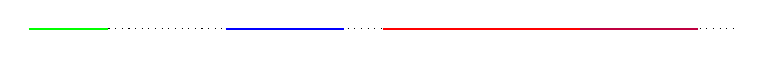
\begin{tikzpicture}[thick, scale=0.1]
      \draw [dotted, thin] (0, 0) -- (90, 0);
      \draw [green] (0, 0) -- (10, 0);
      \draw [blue] (25, 0) -- (40, 0);
      \draw [red] (45, 0) -- (70, 0);
      \draw [purple] (70, 0) -- (85, 0);
    \end{tikzpicture}
\end{center}
\end{figure}
%%% Local Variables:
%%% mode: latex
%%% TeX-master: "../rapportGp1"
%%% End:


%%% Local Variables:
%%% mode: latex
%%% TeX-master: "../rapportGp1"
%%% End:
